%==================================================================================
%==================================================================================
% Document		:		Chapitre: Résumé automatique
%
% Auteur		: 		Abdelkrime ARIES
% Encadreur		:		Dr. Omar NOUALI
% Co-encadreur	:		Mme. Houda OUFAIDA
% Établissement	:		ESI (Ecole Nationale Supérieure d'Informatique; ex. INI) 
% Adresse		:		Oued Smar, Alger, Algérie 
% Année			:		2012/2013
% Grade			:		Magister
% Discipline 	:		Informatique 
% Spécialité	:		IRM (Informatique Répartie et Mobile)
% Titre			:		Résumé automatique de textes
%
%==================================================================================
%==================================================================================

%==========================L'entete de chapitre====================================
%==================================================================================
 \ifx\wholebook\relax\else
  	\documentclass[a4paper,12pt,oneside]{../use/ESIthesis}
  	
  	\usepackage{amsmath,amssymb}             % AMS Math
\usepackage[utf8]{inputenc}
%\usepackage[T1]{fontenc} %,LAE 
\usepackage[T1]{fontenc}
%\usepackage[french,english]{babel}
\usepackage[frenchb]{babel}
\usepackage{microtype}

%\usepackage[left=2.5cm,right=2.5cm,top=2.5cm,bottom=2.5cm,includefoot,includehead,headheight=13.6pt]{geometry}
\usepackage[left=2.8cm,right=2.2cm,top=2.8cm,bottom=2.8cm,includefoot,includehead,headheight=13.6pt]{geometry}
%\usepackage[left=3.8cm,right=3.2cm,top=2.8cm,bottom=2.8cm,includefoot,includehead,headheight=13.6pt]{geometry}
%\usepackage[left=1.5in,right=1.3in,top=1.1in,bottom=1.1in,includefoot,includehead,headheight=13.6pt]{geometry}
\renewcommand{\baselinestretch}{1.5}

% Table of contents for each chapter

\usepackage[nottoc, notlof, notlot]{tocbibind}
\usepackage[french]{minitoc}
\setcounter{minitocdepth}{1}
\mtcindent=15pt
% Use \minitoc where to put a table of contents

\usepackage{aecompl}

% Glossary / list of abbreviations

\usepackage[intoc]{nomencl}
%\renewcommand{\nomname}{List of Abbreviations}

\makenomenclature

% My pdf code

\usepackage[pdftex]{graphicx}
\usepackage[a4paper,pagebackref,hyperindex=true]{hyperref}

%I added
%\usepackage{tabulary}
%\usepackage{longtable}
%\usepackage[table]{xcolor}
\usepackage{indentfirst}


% Links in pdf
\usepackage{color}
%\definecolor{linkcol}{rgb}{0,0,0.4} 
%\definecolor{citecol}{rgb}{0.5,0,0} 

% Change this to change the informations included in the pdf file

% See hyperref documentation for information on those parameters

\hypersetup
{
%bookmarksopen=true,
pdftitle=Résumé Automatique de Textes,
pdfauthor=Abdelkrime ARIES, 
pdfsubject= {Résumé automatique de textes en utilisant une approche statistique, le regroupement, et la classification} , %subject of the document
%%pdftoolbar=false, % toolbar hidden
%pdfmenubar=true, %menubar shown
%pdfhighlight=/O, %effect of clicking on a link
colorlinks=false, %couleurs sur les liens hypertextes
%pdfpagemode=None, %aucun mode de page
%pdfpagelayout=SinglePage, %ouverture en simple page
%pdffitwindow=true, %pages ouvertes entierement dans toute la fenetre
%linkcolor=linkcol, %couleur des liens hypertextes internes
%citecolor=citecol, %couleur des liens pour les citations
%urlcolor=linkcol %couleur des liens pour les url
}



% Some useful commands and shortcut for maths:  partial derivative and stuff

\newcommand{\pd}[2]{\frac{\partial #1}{\partial #2}}
\def\abs{\operatorname{abs}}
\def\argmax{\operatornamewithlimits{arg\,max}}
\def\argmin{\operatornamewithlimits{arg\,min}}
\def\diag{\operatorname{Diag}}
\newcommand{\eqRef}[1]{(\ref{#1})}

\usepackage{rotating}                    % Sideways of figures & tables
%\usepackage{bibunits}
%\usepackage[sectionbib]{chapterbib}          % Cross-reference package (Natural BiB)
%\usepackage{natbib}                  % Put References at the end of each chapter
                                         % Do not put 'sectionbib' option here.
                                         % Sectionbib option in 'natbib' will do.
\usepackage{fancyhdr}                    % Fancy Header and Footer

\usepackage{txfonts}                     % Public Times New Roman text & math font
  
%%% Fancy Header %%%%%%%%%%%%%%%%%%%%%%%%%%%%%%%%%%%%%%%%%%%%%%%%%%%%%%%%%%%%%%%%%%
% Fancy Header Style Options

\pagestyle{fancy}                       % Sets fancy header and footer
\fancyfoot{}                            % Delete current footer settings

%\renewcommand{\chaptermark}[1]{         % Lower Case Chapter marker style
%  \markboth{\chaptername\ \thechapter.\ #1}}{}} %

%\renewcommand{\sectionmark}[1]{         % Lower case Section marker style
%  \markright{\thesection.\ #1}}         %
%\fancyhead[LE,RO]{\bfseries\thepage}    % Page number (boldface) in left on even
%										% pages and right on odd pages
%\fancyhead[RE]{\bfseries\nouppercase{\leftmark}}      % Chapter in the right on even pages
%\fancyhead[LO]{\bfseries\nouppercase{\rightmark}}     % Section in the left on odd pages

\fancyhead[R]{\bfseries\thepage}    % Page number (boldface) in right
\fancyhead[L]{\bfseries\nouppercase{\rightmark}}     % Section in the left on odd pages

\let\headruleORIG\headrule
\renewcommand{\headrule}{\color{black} \headruleORIG}
\renewcommand{\headrulewidth}{1.0pt}
\usepackage{colortbl}
\arrayrulecolor{black}

\fancypagestyle{plain}{
  \fancyhead{}
  \fancyfoot{}
  \renewcommand{\headrulewidth}{0pt}
}

%\usepackage{algorithm}
%\usepackage[noend]{algorithmic}

%%% Clear Header %%%%%%%%%%%%%%%%%%%%%%%%%%%%%%%%%%%%%%%%%%%%%%%%%%%%%%%%%%%%%%%%%%
% Clear Header Style on the Last Empty Odd pages
\makeatletter

\def\cleardoublepage{\clearpage\if@twoside \ifodd\c@page\else%
  \hbox{}%
  \thispagestyle{empty}%              % Empty header styles
  \newpage%
  \if@twocolumn\hbox{}\newpage\fi\fi\fi}

\makeatother
 
%%%%%%%%%%%%%%%%%%%%%%%%%%%%%%%%%%%%%%%%%%%%%%%%%%%%%%%%%%%%%%%%%%%%%%%%%%%%%%% 
% Prints your review date and 'Draft Version' (From Josullvn, CS, CMU)
\newcommand{\reviewtimetoday}[2]{\special{!userdict begin
    /bop-hook{gsave 20 710 translate 45 rotate 0.8 setgray
      /Times-Roman findfont 12 scalefont setfont 0 0   moveto (#1) show
      0 -12 moveto (#2) show grestore}def end}}
% You can turn on or off this option.
% \reviewtimetoday{\today}{Draft Version}
%%%%%%%%%%%%%%%%%%%%%%%%%%%%%%%%%%%%%%%%%%%%%%%%%%%%%%%%%%%%%%%%%%%%%%%%%%%%%%% 

\newenvironment{maxime}[1]
{
\vspace*{0cm}
\hfill
\begin{minipage}{0.5\textwidth}%
%\rule[0.5ex]{\textwidth}{0.1mm}\\%
\hrulefill $\:$ {\bf #1}\\
%\vspace*{-0.25cm}
\it 
}%
{%

\hrulefill
\vspace*{0.5cm}%
\end{minipage}
}

\let\minitocORIG\minitoc
\renewcommand{\minitoc}{\minitocORIG \vspace{1.5em}} %1.5em

\usepackage{multirow}
%\usepackage{slashbox}

\newenvironment{bulletList}%
{ \begin{list}%
	{$\bullet$}%
	{\setlength{\labelwidth}{25pt}%
	 \setlength{\leftmargin}{30pt}%
	 \setlength{\itemsep}{\parsep}}}%
{ \end{list} }

\newtheorem{definition}{Définition }
\renewcommand{\epsilon}{\varepsilon}

% centered page environment

\newenvironment{vcenterpage}
{\newpage\vspace*{\fill}\thispagestyle{empty}\renewcommand{\headrulewidth}{0pt}}
{\vspace*{\fill}}

%%%%%%%%%%%%%%%%%%%%%%%%%%%%%%%%%%%%%%%%%%%%%%%%%%%%%%%%%%%%%%%%%%%%
% Par Karim
%%%%%%%%%%%%%%%%%%%%%%%%%%%%%%%%%%%%%%%%%%%%%%%%%%%%%%%%%%%%%%%%%%%%
%for the degree sign
\usepackage{textcomp} 
\usepackage{bookmark}
\usepackage{framed}
\usepackage{arabtex}
%\usepackage{nashbf}
%\usepackage{atrans}
%calligra font for the remerciement
\usepackage{calligra}

%List of acronyms
\usepackage{acronym}

\newcommand{\racine}{./}

\newcommand{\setracine}[1]{\renewcommand{\racine}{#1}}

\newcommand{\tablefile}[1]{\input{\racine tab/#1}}
\newcommand{\appendixfile}[1]{\input{\racine anx/#1}}
%\newcommand{\chapterfile}[1]{\input{\racine chap/#1}}

\newcommand{\stitle}[1]{
\noindent
\textbf{#1}
}

\newenvironment{itemizeb}
{\begin{list}{\textbullet} {\setlength{\rightmargin}{0cm} \setlength{\leftmargin}{1cm}}}
{\end{list}}


\newenvironment{itemizec}
{\begin{list}{\textopenbullet} {\setlength{\rightmargin}{0cm} \setlength{\leftmargin}{1cm}}}
{\end{list}}


\newcommand{\kexpbox}[1]{

\vspace{5mm}
\noindent
 \fbox{%
   \parbox{0.985\linewidth}{%
   \vspace{2mm}
   {\large  \textbf{Exemple:}}\\
      #1
   }%
 }
}

\newcommand{\kbox}[1]{

\vspace{2mm}
\noindent
 \fbox{%
   \parbox{0.965\linewidth}{%
   \vspace{2mm}
      #1
   }%
 }
}

\newenvironment{kexp}
{
\begin{framed}
\noindent
{\large  \textbf{Exemple:}}\\
}
{
\end{framed}
}

%%%%%%%%%%%%%%%%%%%%%%%%%%%%%%%%%%%%%%%%%%%%%%%%%%%%%%%%%%%%%%%%%%%%
%%%%%%%%%%%%%%%%%%%%%%%%%%%%%%%%%%%%%%%%%%%%%%%%%%%%%%%%%%%%%%%%%%%%

% definitions.
% -------------------

\setcounter{secnumdepth}{3}
\setcounter{tocdepth}{2}

\newcommand{\tab}[1]{{\hskip #1}}
  	 	
  	 	\setracine{../}
  	 	\graphicspath{{.}{../fig/}}

  	 	\begin{document}
  	 	
  	 	\dominitoc 
  	 	\selectlanguage {francais}
  	 	%just to create the .toc file, then you can hide it
  	 	%\tableofcontents
  	 	\mainmatter
  \fi
%==================================================================================

\chapter{Résumé automatique}%
\label{chap:RA}
\minitoc
	
%feature = critère, caractéristique, aspect, indicateur, métrique, trait, facteur
%========================01========================%
%==================================================%
\section{Introduction}

Le résumé automatique de documents n'est pas un nouveau domaine. 
Dès les années 50, les chercheurs font leurs études sur le développement d'un outil permettant de résumer les documents, en utilisant des différentes méthodes pour améliorer ce résumé. 
De ce fait, plusieurs approches sont apparaît pour le résumé automatique de documents. 

Dans ce chapitre, nous allons introduire le résumé automatique de documents d'une manière générale. 
Premièrement, nous allons voir quelques définitions pour la fonction de résumé. 
Ensuite, nous allons présenter les différents types du résumé automatique en se basant sur trois critères: selon le document d'entrée, selon l'objectif, et selon le document de sortie. 
Après, nous allons présenter les étapes du résumé automatique ainsi que les deux approches les plus connus: l'approche statistique et l'approche linguistique. 
%Pour mieux comprendre comment les applications de résumé automatique se fonctionnent, la procédure de résumé automatique va être présentée. 
Enfin, nous allons présenter les différentes applications du résumé automatique, ainsi que quelques outils industriels. 

%========================01========================%
%==================================================%
\section{Définition}

Dans \cite{95-kupiec-al}, le résumé est définit comme: 
"Résumer est de réduire la complexité y compris la taille, avec la conservation de quelques qualités essentielles dans l'original". 
Les auteurs considèrent les titres, les mots-clés, les tables du contenu et les abstraits comme des formes du résumé, 
quand un résumé réfère conventionnellement à une condensation du document entier, similaire aux abstraits.

Ainsi, les auteurs de \cite{02-radev-al} définissent un résumé comme "\textit{un texte produit d'un ou plusieurs textes, 
qui contient les informations importantes du (des) texte(s) original (originaux),
et qui est moins que la moitié du (des) texte(s) original (originaux) et habituellement trop moins que çà}".
Dans cette définition, on peut apercevoir trois aspects importants qui caractérisent le résumé automatique:
\begin{itemize}
\item Les résumés peuvent être produits d'un ou plusieurs documents,
\item Les résumés doivent préserver les informations importantes,
\item Les résumés doivent être courts.
\end{itemize}

Une autre définition est celle du standard de documentation \textbf{ISO}, un résumé de conclusion est "\textit{un bref exposé dans un document (généralement placé à la fin de ce document) de ses découvertes et de ses conclusions caractéristiques, et qui a comme but de compléter l'orientation de lecteur qui a étudié le texte précédent}" \cite{02-minel}, quand un abstrait est "\textit{Une représentation courte du contenu de document sans interprétation ou criticisme}". 
Ainsi, un abstrait est souvent placé dans le début du texte, par exemple dans un rapport scientifique \cite{07-hassel}.
D'après Le Petit Larousse 2009, le résumé est une "\textit{forme condensée d'un texte, d'un discours, etc. ; abrégé, sommaire}". 

%========================01========================%
%==================================================%
\section{Classification de résumé automatique}

La classification du résumé automatique peut varier selon le critère choisi pour la faire. 
C'est pour cette raison, le résumé automatique n'appartient pas exclusivement à une classe donnée, et donc on peut trouver un résumé qui appartient à plusieurs classes. 
Tout résumé peut être classifié par (au moins) trois classes majeures des facteurs de classification \cite{98-hovy-lin}. 
Selon \cite{99-sparckjones} et \cite{98-hovy-lin}, on peut classifier ces facteurs en trois catégories: des facteurs sur document d'entrée, des facteurs sur l'objectif, et des facteurs sur le document de sortie. 
La figure \ref{fig:classif-resume} illustre les différents facteurs de classification.

\begin{figure}[ht]
\begin{center}
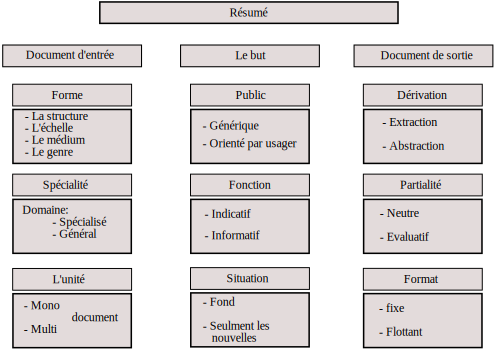
\includegraphics{RA/classif-resume.pdf} % % %[width=140mm]
 \caption{Les différentes classes d'un résumé automatique.}
 \label{fig:classif-resume}
\end{center}
\end{figure}

\subsection{Le document d'entrée}

Les documents utilisés comme entrée d'un système de résumé automatique, peuvent prendre plusieurs formes. 
Ils peuvent aussi être spécialisés pour un domaine, comme ils peuvent appartenir à des domaines arbitraires. 
Si ces documents ont le même thème, on peut les prendre tous comme entrée, alors un système de résumé peut être mono-document ou multi-document. 
Donc, on peut déduire qu'il existe trois façons de classifier le résumé en fonction du document d'entrée: selon sa forme, selon sa spécialité, et selon l'unité.

\subsubsection{La forme}

La forme contient plusieurs aspects: la structure, l'échelle, le médium, et le genre. 
La structure comprend l'organisation explicite comme le marquage par des entêtes (exp. l'objectif, data, méthode, etc.), 
et aussi la structure introduite dans le document comme les modèles rhétoriques familiers (exp. une déclaration suivi d'une élaboration). 
Il est plus approprié ou non de préserver la structure de document dans le résumé. 
En prenant les articles scientifiques comme un exemple, la structure commune dans ce type de document contient les composants: l'introduction, les travaux reliés, le travail réalisé, l'évaluation, et la conclusion. 
Si on ne veut pas préserver la structure de ce document, on peut simplement faire un résumé sur son contenu entier. 
Sinon, le résumé va avoir comme contenu, le résumé de chaque composant du document d'entrée. 
Le travail de \cite{93-paice-jones} est un exemple des travaux qui prennent en considération la structure du document. 
Il utilise comme documents d'entrée, les papiers de recherche très structurées en examinant un corpus des articles pour en extraire les différents patterns des structures existantes. 
Il y a aussi le travail de \cite{04-farzindar-al}, qui traite les textes juridiques en se basant sur leur structure qui comporte quatre thèmes: INTRODUCTION, CONTEXTE, RAISONNEMENT JURIDIQUE et CONCLUSION. 

Du fait qu'on peut résumer un paragraphe comme on peut résumer un livre, l'échelle est importante puisqu'elle contient l'implication pas seulement pour le degré de réduction de résumé, mais aussi pour l'ampleur possible de la transformation du contenu. 
Ainsi, un roman très long peut être aperçu et présenté dans un résumé plus qu'un petit article de nouvelles. 
Un des exemples sur la petite échelle est le travail de \cite{06-kazantseva} dont l'objectif était de résumer les histoires courtes afin d'aider le lecteur à déterminer s'il est intéressé ou non par l'histoire, en fournissant une idée sur les paramètres de cette histoire (comme les caractères, heure, lieu, etc.) sans donner de détails.

Le médium est le support du document d'entrée. 
En regardant aux recherches sur le résumé automatique, on trouve que le support le plus utilisé est le texte, bien qu'il existe d'autres supports comme l'image, le son, la vidéo, etc. 
Ces supports contiennent des informations qu'on peut extraire et résumer de même principe que celui du document texte. 
Parmi les travaux qui concernent le résumé d'un document non textuelle, on peut citer: le résumé des enregistrements audio \cite{01-hori-furui} et \cite{04-Inoue-al}, résumé des vidéos comme dans \cite{03-ekin-al} et \cite{06-albanese-al} qui ont comme but de résumer des vidéo concernant le football, ou des images comme dans le travail de \cite{02-carson-al} et \cite{03-feifei-al}.

%Les genres typiques d'une entrée sont les articles de journaux, les pièces d'opinion, les romans, les histoires, les livres, les rapports, etc. 
Différentes techniques de résumés peuvent être appliquées sur différents genres selon différents échelles, et pas sur d'autres. 
Ces genres peuvent âtre des articles de journaux, des pièces d'opinion, des romans, des histoires, des livres, des rapports, etc. 
%Le travail de \cite{06-kazantseva} est un exemple sur un genre spécifique sur l'entrée; il prend comme entrée, les histoires courtes. 
Un exemple est celui de \cite{09-zhan-al} qui prend comme entrée les documents de genre pièces d'opinion (en Anglais: \textit{reviews}).

\subsubsection{La spécialité}

%Selon la spécialité du résumé par rapport aux documents utilisés, on peut considérer le résumé automatique comme étant de type domaine spécialisé ou générale. 
Le résumé automatique peut être général ou spécifique à un domaine précis. 
Lorsque les documents d'entrée ont tous le même domaine, il est plus approprié d'utiliser un système de résumé automatique spécialisé pour ce domaine. 
Donc, ce type de résumé peut diminuer le degré d'ambiguïté des termes, les mots particuliers et usage de grammaire, et le formatage spécialisé.
%Ceci le rendre plus approprié pour les résumés par abstraction (génération) \cite{93-mitkov}.
Un des exemples sur un résumé de domaine spécifique est le travail de \cite{07-reeve-al} qui s'intéresse aux textes biomédicaux pour aider les médecins à lire les informations concernant les tests cliniques des patients. 
Dans le domaine de droit, on peut citer le travail de \cite{04-farzindar-al}, qui prend en entrée des textes juridiques afin de permettre aux juristes de consulter rapidement les idées clés d'une décision juridique et trouver les jurisprudences pertinentes à leurs besoins.

D'autre part, un résumé de domaine général est dérivé d'un ou plusieurs documents d'entrée dans n'importe quel domaine. 
Un exemple de résumé de domaine générale est donné par le travail de \cite{03-nomoto-matsumoto} qui peut être appliqué pour n'importe quelle domaine, en exploitant la diversité des concepts dans le document d'entrée.

\subsubsection{L'unité}

Selon le nombre de sources, on peut classifier le résumé automatique de documents en deux catégories: Mono-document et multi-documents. 
Un résumé mono-document est un résumé qui traite un seul document en entrée (même si le processus utilise des données compilées antérieurement d'autres documents). 
Il existe plusieurs recherches sur le résumé automatique mono-document, commençant par le travail de Luhn \cite{58-luhn}. 
Parmi ces travaux, on peut prendre comme exemple: \cite{69-edmundson}, \cite{93-mitkov}, \cite{95-kupiec-al}, \cite{98-hovy-lin}, \cite{04-farzindar-al}, etc.

D'autre part, un résumé multi-documents est un résumé qui couvre le contenu de plusieurs documents en entrée, et qu'il est utilisé seulement si ces documents sont reliés par un même thème. 
Il parait que ce type de résumé a été utilisé pour la première fois par \cite{95-mckeown-radev}, en développant le système SUMMONS\footnote{SUMMONS: SUMMarizing Online NewS articles}. %\cite{07-das-martins}. 
Un exemple sur le résumé multi-documents est le travail de \cite{09-boudin-torresmoreno} qui se considère comme le premier travail qui contient une évaluation d'une approche de résumé automatique multi-documents sur les textes en français. 

\subsection{Le but}

Un système de résumé peut être générique où le résumé toujours procède de la même façon quelque-soit l'utilisateur, ou il peut être contrôlé par l'utilisateur. 
Il peut être destiné pour indiquer seulement une idée sur le document sans donner aucun contenu, comme il peut être destiné pour informer l'utilisateur sur le contenu du document, en fournissant une version courte.
Il peut fournir un résumé détaillé en supposant que l'utilisateur n'a aucune connaissance préalable du thème, ou juste fournir les nouvelles.
Donc, selon le but de résumé, on obtient trois facteurs de classification : le public, la fonction, et la situation. 
% Ils sont les facteurs les plus importants selon \cite{99-sparckjones}, puisqu'ils sont critiques, leurs implications peuvent s'étendre, et ils sont la base d'évaluation.

\subsubsection{Le public}

Selon le public, on peut classifier le résumé sur deux catégories: générique et orienté par requête (profil utilisé). 
Un résumé générique est un résumé qui fournit le point de vu de l'auteur (les auteurs) sur un ou plusieurs documents d'entrée, en donnant la même importance pour tous les thèmes majeurs. 
Autrement dit, il ne tient pas compte de ce que l'utilisateur veut chercher. 
Il existe plusieurs exemples sur ce type de résumé, parmi eux on trouve \cite{06-kazantseva}.
%\cite{05-usunier-al} donne une méthode statistique pour le résumé automatique à base d'apprentissage qui extraie les phrases pertinentes d'un document. 
%Ce choix n'implique pas qu'on ne peut pas utiliser la requête d'utilisateur dans sa méthode.
Le but dans ce travail est de fournir au lecteur un bref résumé sur une histoire donnée. 
L'utilisateur dans ce travail est supposé chercher sur le thème général de l'histoire, pour juger s'il veut la lire ou non. 
Si on utilise un résumé orienté par requête, donc l'utilisateur doit savoir préalablement ce qu'il cherche, et le but devient absurde. 
%Donc, on peut conclure qu'il existe des travaux dont le but ne nous permet pas d'utiliser un résumé orienté par requête.

Un résumé orienté par requête (ou orienté utilisateur) préfère des thèmes spécifiques ou aspect(s) de document, en répondant sur les envies des utilisateurs pour chercher seulement sur ces thèmes en particulier. 
Il peut être explicite, en sélectionnant les thèmes pertinents. 
Comme il peut être implicite, en négligeant les thèmes qui ne sont pas en relation avec les intérêts de l'utilisateur. 
%Un exemple sur le résumé dirigé par une requête est le travail par \cite{05-usunier-al} qui est un système de résumé automatique couplé à un moteur de recherche, pour permettre aux utilisateurs d'évaluer rapidement la pertinence réelle d'un document par rapport à leur requête. 
Le travail de \cite{09-liu-al} contient une sorte de résumé par requête, lorsque l'utilisateur sélectionne un mot-clé un résumé s'affiche suivant le thème concernant ce mot-clé.

\subsubsection{La fonction}

Selon la fonction, le résumé peut être indicatif ou informatif. 
Le résumé indicatif fournit seulement une indication sur la matière du sujet principal ou le domaine de document(s) d'entrée sans introduire son contenu. 
D'après \cite{04-crispino-couto}, "\textit{un résumé indicatif peut être considéré comme une aide à l'utilisateur pour juger la pertinence du document et l'intérêt qu'il pourrait y avoir à lire le texte original}".
La recherche des mots-clés et thème d'un document est considérée comme une sorte de résumé indicatif, le travail de \cite{09-liu-al} en est un exemple. 
Ce travail est destiné pour aider les utilisateurs à analyser une grande quantité de textes, en fournissant les mots-clés et les thèmes, présentés d'une manière graphique et distribués au long du temps. 
Leur système a été appelé par TIARA\footnote{TIARA: Text Insight via Automated, Responsive Analysis}, une illustration sur la présentation graphique est donnée dans la figure \ref{fig:tiara}.
\begin{figure}[ht]
\begin{center}
\includegraphics[width=140mm]{RA/tiara.pdf} % % %[width=140mm]
 \caption[Un résumé de 10,000 emails dans l'année 2008, créé par TIARA]{Un résumé de 10,000 emails dans l'année 2008, créé par TIARA \cite{09-liu-al}.}
 \label{fig:tiara}
\end{center}
\end{figure}

Un résumé informatif reflet le contenu (ou une partie), et nous permet de décrire le contenu du document d'entrée. 
D'après \cite{04-crispino-couto}, "\textit{Un résumé informatif fournit une information sur tous les points importants du document en cherchant à couvrir tous les sujets traités par le document}".
Ainsi, après la lecture d'un résumé informatif, on peut expliquer sur quel sujet le document d'entrée peut-être, mais pas nécessairement qu'est-ce qu'il peut contenir. 
Deux exemples sur le résumé informatif sont: \cite{09-boudin-torresmoreno} pour le résumé multi-documents et \cite{05-usunier-al} pour le résumé mono-document.

\subsubsection{La situation}

Le résumé selon la situation peut être un résumé de fond (\textit{background}) ou un résumé qui rapporte Seulement-les-nouvelles. 
Un résumé de fond suppose que la connaissance antérieure de lecteur sur le cadre général du contenu de document(s) d'entrée est très pauvre, et donc il inclut des matériels d'explication, comme la situation des places, le temps, et les acteurs. 
Le travail de \cite{06-kazantseva} peut être considéré comme un résumé automatique de fond, puisqu'il assume l'absence de connaissance préalable du lecteur sur le document d'entrée, et donne des informations sur le temps, les places, les caractères, etc.

Un résumé de type Seulement-les-nouvelles contient seulement les thèmes nouveaux ou principaux, en supposant que le lecteur a un fond suffisant pour les interpréter dans le contexte.
% il peut s'appliquer sur le multi-documents surtout. 
Le travail de \cite{10-bysani} présente un système de résumé automatique qui détecte les nouveau thèmes après une période de temps. 
Il est considéré comme un système de résumé multi-documents; qui détecte la nouveauté dans un document par rapport aux documents passés.

\subsection{Le document de sortie}

Le résumé d'un document peut être obtenu de deux manières: la première est de prendre les phrases (ou des parties) qu'elles semblent plus probable de représenter ce document, la deuxième est de générer le résumé. 
Il peut refléter le document d'entrée sans introduire des jugements, comme il peut porter des jugements sur son contenu.
Tandis que le format du résumé peut être fixe pour tous les documents d'entrée, comme il peut varier selon les types de ces documents.
Les trois critères de classification, en observant le document de sortie, sont: la dérivation, la partialité, et le format.

\subsubsection{Dérivation}

De ce point de vu, un résumé est soit une extraction ou une abstraction. 
Une extraction est une collection de passages (des mots jusqu'à des paragraphes) extraite d'un document d'entrée et produite textuellement comme un résumé. 
Les premières techniques d'extraction ont utilisé le calcul de score pour chaque phrase en fonction des critères tels que la fréquence de mots de phrase \cite{58-luhn}, la position dans le texte \cite{58-baxendale,69-edmundson}, les phrases clés \cite{69-edmundson}. 
Des méthodes d'extraction récentes utilisent d'autres techniques plus sophistiquées pour décider quelle phrase va être extraite. 
Ces techniques dépendent souvent sur l'apprentissage automatique pour identifier les critères importants, sur l'analyse du langage naturel pour identifier les passages clés, ou sur les relations entre les mots plutôt que des sacs de mots \cite{02-radev-al}.

Une abstraction est un texte (document en général) nouvellement généré, produit de certaines représentations internes, et qui est un résultat de l'analyse de l'entrée. 
Le résumé par abstraction est difficile à concevoir, en le comparant avec le résumé par extraction, mais on peut le rendre moins difficile en utilisant quelques techniques. 
Parmi ces techniques, la conception d'une méthode de résumé destinée à un domaine spécifique des documents, cela rend le processus plus facile, comme il est indiqué par \cite{93-mitkov}. 
Pour éviter le problème de différenciation entre les concepts importants dans le texte entre autres, l'auteur utilise un domaine spécifique pour les documents d'entrée.

\subsubsection{Partialité}

Ce critère est principalement appliqué quand le matériel d'entrée est un sujet d'opinion ou pré-jugement. 
Un résumé selon la partialité peut être neutre ou évaluatif. 
Un résumé neutre reflète le contenu de document(s) d'entrée, soit partialement ou impartialement, sans introduire des critiques ou évaluations. 
La plupart des recherches dans le résumé automatique sont de ce type.

Un résumé évaluatif inclut quelques jugements propres au système, soit explicitement (en utilisant des déclarations d'opinion) ou implicitement (en incluant des matériels d'un pré-jugement et l'omission des matériels avec un autre). 
Le travail de \cite{12-workman-al} représente un système de résumé automatique destiné pour les documents médicales, et combiné avec un outil de décision, afin d'aider les médecins dans leurs décisions. 
Un autre exemple est celui présenté dans \cite{09-genereux-bossard} qui traite les textes d'opinion par l'analyse de blogs, où sont exprimées à la fois des informations factuelles et des prises de position sur les faits considérés.

\subsubsection{Le format}

Un résumé, selon le format, peut être fixe ou flottant. 
Un résumé d'un format fixe est créé pour une utilisation, utilisateur (ou classe d'utilisateurs), ou situation spécifique. 
Comme tel, il peut se conformer aux conventions internes appropriées de soulignement, formatage, etc.

Un résumé d'un format flottant est un résumé ayant un format varié; il est créé et affiché avec des préférences variées, pour des différents utilisateurs, et des différents buts. 
Par exemple, pour un utilisateur donné, le système produit un résumé au format d'une table, et pour un autre utilisateur, pour le même document, il affiche un texte.

%========================01========================%
%==================================================%
\section{Étapes du résumé automatique}

Dans le résumé automatique de documents, on peut identifier trois différentes étapes \cite{98-hovy-lin, 99-sparckjones}. 
La plupart des systèmes aujourd'hui utilisent la première étape seulement. 
Ces étapes sont: l'identification du thème, l'interprétation, et la génération du résumé (voir la figure \ref{fig:proc-resume}). 
L'identification des thèmes produit un résumé simple; une fois le système repère les unités importantes, il les présente comme un extrait. 
Ensuite, l'interprétation qui comporte la fusion des concepts, l'évaluation, ou autres procédures qui utilisent une connaissance autre que le (les) document(s) d'entrée. 
Le résultat de l'interprétation est un abstrait non lisible, ou un extrait incohérent. 
Donc, l'étape de génération sert à produire un texte (document) lisible par l'humain, et dans le cas de l'extrait cette étape peut être considérée comme étape de "lissage" pour rendre le résumé plus cohérent.

\begin{figure}[ht]
\begin{center}
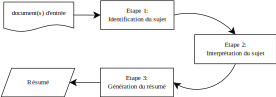
\includegraphics{RA/proc-resume.pdf} % % %[width=140mm]
 \caption{Procédure de résumé automatique.}
 \label{fig:proc-resume}
\end{center}
\end{figure}

\subsection{Étape 1: Identification des thèmes}

Elle sert à produire un résumé simple (extrait) en détectant les unités importantes dans le document (mot, phrase, paragraphes, etc.). 
Les systèmes de résumé qui utilisent seulement l'étape d'identification du thème, produisent un résumé extractif. 
Ceci se fait par filtrage du fichier d'entrée pour obtenir seulement les thèmes les plus importants. 
Une fois ces thèmes identifiés, ils sont présentés sous forme d'un extrait.

Pour effectuer cette étape, presque tous les systèmes utilisent plusieurs modules indépendants. 
Chaque module attribue un score aux unités d'entrée (mot, phrase ou passage plus long), puis un module de combinaison combine les scores pour chaque unité afin d'attribuer un score unique. 
Enfin, le système renvoie les unités du plus haut en score, en fonction de la longueur du résumé, demandé par l'utilisateur ou fixé préalablement par le système.

\subsection{Étape 2: Interprétation des thèmes}

Dans l'interprétation, le but est de faire un compactage en réinterprétant et en fusionnant les thèmes extraits pour avoir des thèmes plus brefs. 
Ceci est indispensable du moment que les abstraits sont généralement plus courts que les extraits équivalents. 
Cette deuxième phase de résumé automatique (passage de l'extrait vers l'abstrait) est naturellement plus complexe que la première. 
Pour compléter cette phase, le système a besoin de connaissances sur le monde (par exemple, les anthologies), puisque sans connaissance aucun système ne peut fusionner les sujets extraits pour produire des sujets moins nombreux afin de former une abstraction. 
Lors de l'interprétation, les thèmes identifiés comme importants sont fusionnés, représentée en des termes nouveaux, et exprimé en utilisant une nouvelle formulation, en utilisant des concepts ou des mots qui n'existent pas dans le document original. 

\subsection{Étape 3: Génération du résumé}

% Introduction à l'étape
Le résultat de l'interprétation est un ensemble de représentations souvent non lisibles, c'est le cas du résumé par abstraction.
Pour le résumé extractif, le résultat est un extrait rarement cohérent, à cause des références coupées, la négligence des liens entre les phrases, et la redondance ou la négligence de quelques matériels. 
De ce fait, les systèmes incluent une étape de génération du résumé afin de produire un texte cohérent et lisible par l'humain. 

% En général: dans le cas de l'abstraction
Dans cette étape, le système a besoin d'utiliser des techniques de la génération de langage naturel qui, selon \cite{98-hovy-lin}, a besoin de deux modules: le micro-planeur et le générateur des phrases. 
Le micro-planeur, dans le contexte du résumé automatique, a comme fonction d'assurer que l'information sélectionnée par les deux étapes précédentes (identification et interprétation du thème) est rédigée d'une manière compacte et brève autant que possible en restant dans un état grammatical. 
Il peut être construit pour mener son travail sur deux niveaux: le niveau textuel et le niveau représentatif. 
Dans le premier niveau, l'entrée est une liste de phrases ou fragments de phrases, et la sortie est une liste compacte de phrases. 
Dans le deuxième niveau, l'entrée est exprimée sous une notation abstraite, et la sortie est une spécification abstraite et syntaxique pour chaque phrase. 
La sortie de ce niveau n'est pas lisible par l'humain c'est pour ça il faut passer par la génération des phrases. 
Un des micro-planeurs destinés pour le résumé automatique est celui de \cite{95-mckeown-radev}.

Le deuxième module est le générateur de phrases, qui transforme une spécification détaillée d'une ou plusieurs unités propositionnelles vers une phrase grammaticalement correct. 
Il existe des générateurs de phrases, qui sont relativement faciles à utiliser, pour les recherches. 
Parmi ces générateurs, il y a Penman \cite{91-hovy}, FUF/SURGE \cite{92-elhadad}, RealPro \cite{97-lavoie-rambow}, et NITROGEN \cite{98-langkilde-knight}. 

Les résumés par extraction n'exigent pas l'étape de génération, mais certaines incohérences vont être observées lorsqu'on extrait des phrases (ou autres unités), et on les assemble en ordre d'importance ou de l'emplacement dans le document. 
Parmi les aspects qui rend le texte incohérent ou non courant, les suivants:
\begin{itemize}
\item La répétition des clauses ou phrases nominales; qui peut être fixée par l'agrégation dans une combinaison.
\item La répétition des entités nommés; qu'on peut fixer en substituant ces entités par des pronoms.
\item L'inclusion des matériels moins importants comme les parenthèses, ceci peut être réglé par la suppression de ces matériels.
\end{itemize}
Dans \cite{99-mani-al2}, les auteurs décrivent un programme de révision du résumé, qui prend en entrée des extraits simples et produit des résumés plus courts et plus lisibles. 
On peut résoudre, aussi, d'autres problèmes d'incohérence qui sont plus difficiles comme les liens anaphoriques cassés, ou les liens entre les phrases et la fluidité du sens. Comme on peut utiliser la compression des phrases afin de rendre le résumé plus court et plus précis.

%========================01========================%
%==================================================%
\section{Approches de résumé automatique}

Il existe deux grandes approches pour le résumé automatique: l'approche statistique et l'approche linguistique. 
L'approche statistique est la plus ancienne, elle revient au années 50 lorsque Luhn a conçu le premier outil du résumé automatique \cite{58-luhn}. 
L'idée d'utiliser l'intelligence artificielle est apparue dans les années 80, pour montrer la capacité de compréhension, c'est ainsi que la méthode linguistique a apparue \cite{02-minel}.

\subsection{L'approche statistique}

L'approche statistique se trouve généralement dans l'étape d'identification de thèmes. 
C'est l'approche la plus ancienne, elle revient au début de recherches sur le résumé automatique dans les années 50. 
Les méthodes statistiques n'utilisent pas de ressources linguistiques, elles sont basées essentiellement sur le calcul d'un score associé à chaque unité (phrase) afin d'estimer son importance dans le texte.

\subsubsection{Le principe}

Le principe de la méthode statistique consiste à sélectionner les unités (phrases) saillantes et les combiner pour avoir un résumé. 
L'approche statistique comprend les trois phases illustrées dans la figure \ref{fig:app-stat}.

\begin{figure}[ht]
\begin{center}
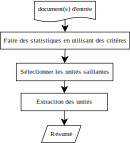
\includegraphics{RA/app-stat.pdf} % % %[width=70mm]
 \caption{Résumé par approche statistique.}
 \label{fig:app-stat}
\end{center}
\end{figure}

La première étape consiste à faire des statistiques sur des critères pour chaque unité (pour un document texte, elle peut être une phrase, un paragraphe, etc.). 
Pour le résumé d'un document texte, ces critères peuvent être: la fréquence des mots, la position des mots, les mots de titre, etc. 
La deuxième phase consiste à sélectionner les unités saillantes dans le texte, en se basant sur les statistiques précédentes, et en attribuant à chaque unité un score selon ces critères. 
Enfin, la phase d'extraction qui consiste à éliminer les unités ayant un score très faible, et donc qui ne sont pas pertinentes dans le document. 
%Cette méthode, ainsi que ses différentes étapes vont être discutés dans le deuxième chapitre.

Le calcul du score de chaque unité se fait en accumulant les poids de chaque critère présent dans cette unité, multiplié par un coefficient spécifique pour ce critère. 
La méthode de calcul du score d'une unité (exp. phrase) $P$ est donnée par l'équation \ref{eq:score-stat}. 
\begin{equation}
\label{eq:score-stat}
Score(P) = \sum_{1 \leq i \leq k} {\alpha_i * C_i(P)}
\end{equation}
Où:
\begin{itemize}
\item $k$ étant le nombre total de critères retenus pour calculer le score de l'unité (exp. phrase);
\item $C_i$ est la fonction calculant la valeur numérique d'un critère $ i $ appliqué à l'unité (exp. phrase);
\item $\alpha_i$ est le coefficient associé au critère $ i $.
\end{itemize}

\subsubsection{Critiques de l'approche statistique}

Les méthodes statistiques sont des méthodes simples, qui attribuent de score en se basant sur certains critères dans le document. 
Il est plus aisé de combiner un ensemble de critères de natures différentes pour exprimer la valeur de pertinence globale d'une phrase (mais aussi d'un paragraphe, etc.).

L'inconvénient majeur de cette méthode est l'incohérence. 
Il existe deux grandes origines de l'incohérence: les anaphores et la structure de phrases. 
Pour les anaphores, on peut trouver dans le résumé un lien anaphorique et qui n'a pas de sens, puisque la phrase qui l'exprime a été éliminée. 
L'autre origine qui est la structure des phrases; lorsqu'on fait l'extraction des phrases, il se peut que les phrases de résumé n'ont aucune relation rhétorique entre elles. 
En plus, on peut trouver dans le résumé des phrases qui sont identiques sémantiquement, et donc un problème de récurrence est vite observé.

%========================01========================%
%==================================================%
\subsection{L'approche linguistique}

%TODO contraduction ??? non pas de contraduction
%pas de contaduction puisque l'approche linguistique peut être extactive comme elle peut être abstractive
L'approche linguistique exploite le savoir linguistique pour générer le résumé, soit par extraction ou par abstraction. 
Elle se passe dans les trois étapes de résumé automatique, précédemment parlé. 
Plusieurs théories entrent dans le cadre de cette approche à savoir : la Théorie de la Structure Rhétorique, et les chaînes lexicales. 
Pour un document (ou plusieurs) d'entrée, le système utilise les informations linguistiques pour créer une représentation de l'entrée. 
Ensuite, cette représentation va être réduite en utilisant des règles de réduction, soit en gardant les phases les plus importantes ou en créant une nouvelle représentation. 
Enfin, l'étape de génération du résumé, qui sert à fusionner les phrases extraites pour avoir un résumé extractif, ou transformer la représentation réduite à un résumé par abstraction. 
La figure \ref{fig:app-ling} illustre les différentes étapes suivies dans l'approche linguistique.
\begin{figure}[ht]
\begin{center}
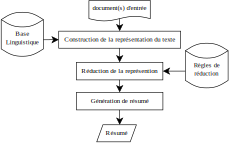
\includegraphics{RA/app-ling.pdf} % % %[width=140mm]
 \caption{Un modèle général pour l'approche linguistique de résumé automatique.}
 \label{fig:app-ling}
\end{center}
\end{figure}

\subsubsection{Les chaînes lexicales}

Dans \cite{97-barzilay-elhadad}, les auteurs ont conduit un travail qui utilise une quantité considérable d'analyse linguistique. 
Ils ont utilisé une méthode qui s'appelle: "chaîne lexicale" (\textit{lexical chain}); définit par une séquence des mots reliés dans un texte, avoir une distance courte (les mots adjacents ou phrases), ou distance longue (le texte entier). 
La production du résumé passe par les étapes suivantes: segmentation du texte, identifications des chaînes lexicales, et l'utilisation des chaînes lexicales puissantes pour identifier les phrases saillantes. 
Ils ont essayé d'atteindre une base entre \cite{95-mckeown-radev} qui effectue une analyse profonde de la structure sémantique du texte, et \cite{58-luhn} qui utilise des statistiques sur les mots du document. 
Les auteurs modélisent la notion de cohésion dans le texte comme une moyenne d'assembler les différentes parties du texte. 
La cohésion lexicale est un exemple où les mots reliés sémantiquement sont utilisés, la phrase suivante illustre cette notion:
\begin{center}
\textit{John a acheté une Peugeot. Il aime les voitures.}
\end{center}
Ici, le mot "voiture" réfère au mot "Peugeot" dans la phrase qui précède, et donne un exemple sur la cohésion lexicale. 
Le phénomène de cohésion ne se passe pas seulement au niveau du mot, mais aussi au niveau des séquences de mots, qui donne des chaînes lexicales. 
Les mots sémantiquement reliés ainsi que les séquences des mots, sont identifiés dans le document, et plusieurs chaînes sont extraites, formant une représentation du document. 
Pour trouver les chaînes lexicales, les auteurs ont utilisé Wordnet \cite{95-miller}, en suivant trois étapes:
\begin{enumerate}
\item Sélection d'un ensemble des mots candidats.
\item Pour chaque mot candidat, trouver la chaîne appropriée en se basant sur un critère de lien entre les membres de la chaîne.
\item S'il existe une chaîne, insérer le mot dans la chaîne et mettre à jour en conséquence.
\end{enumerate}

Le lien est mesuré par la distance dans Wordnet. 
Les noms simples et les noms composés sont utilisés comme point de départ pour trouver l'ensemble des mots candidats dans l'étape 1. 
Enfin, les chaînes lexicales les plus fortes sont utilisées pour créer le résumé. 
Les scores de ces chaînes sont calculés en se basant sur leurs longueurs et homogénéités. 
Puis, les auteurs utilisent quelques heuristiques pour sélectionner les phrases signifiantes. 

\subsubsection{La structure rhétorique}

Dans \cite{94-ono}, les auteurs introduisent un système de génération automatique de résumé pour les discours japonais. 
Ils ont élaboré une procédure pratique pour extraire la structure rhétorique du discours: un arbre binaire représentant les relations entre les parties de la phrase. 
Cette structure a été extraite en utilisant une série d'étapes basées sur le TALN: analyse des phrases, extraction des relations rhétoriques, segmentation, génération de candidat, et jugement de pertinence. 
L'évaluation est basée sur l'importance relative entre les relations rhétoriques.
Dans cette étape, les nœuds de l'arbre représentant la structure rhétorique, sont taillés pour réduire la phrase, en gardant ses parties importantes. 
Le processus est réitéré au niveau des paragraphes afin de produire, finalement, un résumé.
%Evaluation was done with respect to sentence coverage and 30 editorial articles of a Japanese newspaper were used as the dataset. 
%The articles had corresponding sets of key sentences and most important key sentences judged by human subjects. 
%The key sentence coverage was about 51\% and the most important key sentence coverage was 74\%, indicating encouraging results.

\cite{98-marcu} décrit une approche unique pour le résumé automatique qui, au contraire aux autres travaux ultérieurs, ne suppose pas que les phrases dans un document forment une séquence absolue. 
L'auteur utilise les heuristiques basées sur la théorie de structures rhétoriques, combinées avec les critères classiques qui ont été utilisés dans la littérature de résumé automatique. 
Cette théorie repose sur deux concepts: le noyau et le satellite. 
%La théorie du discours utilisée dans cet article est la théorie de structure rhétorique, qui se tient entre deux pièces non superposées de texte: le noyau et le satellite. 
La distinction entre le noyau et le satellite vient de l'observation empirique que le noyau exprime ce qu'il est plus essentiel pour l'objectif de l'auteur que le satellite. 
En plus, le noyau d'une relation rhétorique est compréhensible indépendamment du satellite, mais pas vice versa. 
La figure \ref{fig:arbre-rhet} illustre les relations rhétoriques entre les différentes phrases d'un texte. 
Les chiffres représentent les emplacements des phrases dans le texte, les nœuds pointillés représentent les satellites et les nœuds normaux représentent les noyaux.
\begin{figure}[ht]
\begin{center}
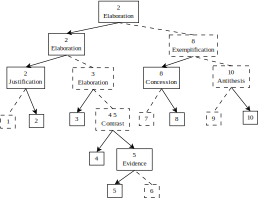
\includegraphics{RA/arbre-rhet.pdf} % % %[width=140mm]
 \caption[Exemple d'une arbre de discours]{Exemple d'une arbre de discours \cite{98-marcu}.}
 \label{fig:arbre-rhet}
\end{center}
\end{figure}

\subsubsection{Critiques de l'approche linguistique}

L'utilisation de cette approche nous garantit une analyse plus profonde du texte d'entrée; on peut examiner les liens sémantiques entre les mots (les synonymes, les antonymes), le sens des phrases, les différents concepts existants et les relations entre eux, etc. 
Un autre point fort de cette approche, est le respect de l'acheminement de l'auteur; on peut extraire les différentes idées existantes dans le texte et générer un résumé qui respecte leur évolution.

Cependant, cette approche reste très lourde, à cause de l'utilisation de traitement de langage naturel qui consomme beaucoup de ressources. 
En plus, les outils de TALN existants ne sont pas assez performants, ainsi l'utilisation de plusieurs outils peut introduire des erreurs de traitement. 
Un autre obstacle pour cette approche est la dépendance du texte d'entrée, donc les méthodes développées par cette approche ne peuvent pas être générales, elles doivent être destinée pour une langue spécifique et/ou un genre déterminé. 

%========================01========================%
%==================================================%
\section{Applications du résumé automatique}

Avec l'augmentation considérable du volume des informations sur Internet, il est devenu très difficile de sélectionner l'information pertinente. 
L'information est publiée simultanément sur plusieurs canaux média avec des versions variantes, par exemple, un journal papier, un journal web, message SMS, des nouvelles de radio, etc. 
La personnalisation de l'information pour les différents canaux et formats est une fonction d'édition immense qui demande notamment de raccourcir le texte original.

Le résumé automatique apporte une solution à ce problème et automatise complètement ce travail. 
En plus, les documents deviennent accessibles par d'autres langues en les résumant premièrement avant traduction, ceci peut être, dans la plupart des cas, suffisant pour juger de la pertinence d'un document avec une langue étrangère. 
De ce fait, on peut éviter le travail de traduction de tout le document manuellement. 
Le résumé automatique peut être utilisé pour résumer un texte avant qu'un synthétiseur de parole automatique le lit, de ce fait on peut réduire le temps nécessaire pour extraire les données clés dans le document. 
En particulier, il peut être utilisé pour préparer l'information pour être utilisée dans les petites appareilles mobiles, comme les PDA, dont le besoin d'une réduction considérable du contenu est nécessaire.

D'après l'institut national américain de normalisation (ANSI): "\textit{Un résumé bien préparé permet aux lecteurs d'identifier le contenu de base d'un document rapidement et avec précision, afin de déterminer sa pertinence pour leurs intérêts, et donc de décider s'ils ont besoin pour lire le document dans son intégralité}" \cite{07-hassel}. 
En effet, le résumé s'avère très bénéfique dans plusieurs tâches d'acquisition d'information, quelques exemples sont donnés dans \cite{75-borko-bernier}:
\begin{itemize}
\item Les résumés permettent d'économiser le temps de lecture;
\item Les résumés facilitent la sélection;
\item Les résumés facilitent les recherches documentaires;
\item Les résumés améliorent l'efficacité d'indexation;
\item Les résumés aident dans la préparation des revues.
\end{itemize}

Parmi les exemples de l'utilisation de résumé, le travail de \cite{07-yang-wang} qui présente un modèle de résumé de documents web pour les appareils portables. 
Le modèle est basé sur la théorie des fractales, il génère un résumé squelette. 
Ensuite, si l'utilisateur veut voir plus de détail, le système génère des niveaux de détails. 
Un autre exemple est celui de \cite{09-zhan-al}, qui se repose sur le résumé des critiques sur les produits. 
Ceci peut aider les sociétés pour développer les modèles conceptuels, la personnalisation, la recommandation des produits, comprendre le client, et, par conséquent, attirer plus de clients.
Dans l'aide à la décision médical, on peut citer le travail de \cite{12-workman-al}, qui utilise un système de résumé automatique pour améliorer la décision médicale. 
Le travail de \cite{11-uzzaman-al} introduit une idée d'illustrer automatiquement les phrases complexes, en utilisant des résumés qui combinent les images, les structures et des textes simples. 

%TODO Done: ccl sur les domaines d'utilisations multiples et variés
Les domaines d'utilisation de résumé automatique sont multiples et variés, ce qui preuve le besoin de développer des outils pour ça. 
Dans la section suivante, nous allons parler sur quelques outils industriels qui aident l'utilisateur à satisfaire les applications citées précédemment.

%========================01========================%
%==================================================%
\section{Outils industriels}

Pour appliquer les domaines d'utilisation précédemment cités, il faut des outils permettant le résumé automatique. 
Il existe plusieurs outils industriels du résumé automatique de documents. 
Certains de ces outils sont commerciaux, d'autres sont gratuits ou open source. 
Nous allons citer quelques exemples sur ses outils destinés pour le résumé automatique de textes.

\subsection{Essential Summarizer} %Pertinence

Essential Summarizer\footnote{Site web: \url{http://www.essential-mining.com}} est un outil de construction de résumés informatifs pour des textes écrits dans différentes langues (Anglais, français, allemand, Italien, etc.) qui se décline en deux versions. 
La première est conçue pour être incorporé dans des Intranets d'entreprise. 
L'autre version est une application de bureautique traditionnelle destinée à l'utilisation personnelle.

Les deux versions sont fondées sur les travaux de recherche de Lehmam \cite{10-lehmam} et s'appuient sur un même noyau informatique programmé en Java, ce qui facilite la portabilité entre les différentes plateformes matérielles. 
Différents formats d'entrée pour les textes sont traités: ASCII, PDF, Word, RTF, et HTML. 

Le programme est développé en se basant sur l'idée que le lecteur va payer plus d'attention à certaines passages du texte puisqu'elles contiennent les informations que lui intéresse. 
Il utilise des techniques linguistiques pour extraire ces informations: 
\begin{itemize}
\item La reconnaissance d'indices sémantiques appelés marqueurs d'extraction sémantique (MLE) afin d'évaluer la pertinence des phrases isolées et des paragraphes entiers;
\item La spécialisation par domaine, afin de mieux cibler le résumé;
\item La prise en considération des expressions ou des concepts qui sont importants pour les besoins de l'utilisateur;
\item Observation de résumés manuels de textes représentatifs, et analyse de retour d'information (feedback) des utilisateurs.
\end{itemize}
Les  connaissances linguistiques sont stockées dans la base des marqueurs linguistiques d'extraction (MLE) – différentes pour chacune des langues traitées – qui sont des expressions linguistiques auxquelles sont affectées des valeurs. 
La base globale des MLE se décompose au niveaux suivants (voir la figure \ref{fig:lehmam-ling}):
\begin{itemize}
\item Marqueurs linguistiques d'extraction indépendants de tout domaine (MLE généraux);
\item MLE propres à un domaine (médicale, financier, etc.);
\item La terminologie propre au domaine;
\item Mots ou expressions utilisateur;
\item Mots ou expressions d'exclusion.
\end{itemize}

\begin{figure}[ht]
\begin{center}
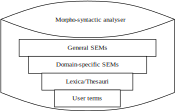
\includegraphics{RA/lehmam-ling.pdf} % % %[width=80mm]
 \caption[Organisation de marqueurs linguistiques]{Organisation de marqueurs linguistiques \cite{10-lehmam}.}
 \label{fig:lehmam-ling}
\end{center}
\end{figure}

L'objectif du système est de repérer les marqueurs de la base des MLE dans le texte à résumer afin de pondérer l'ensemble des phrases du texte. 
Chaque phrase se voit associer un poids qui est la somme des poids des marqueurs linguistiques qu'elle contient. 
Les phrases dont le poids est nul ou très faible sont alors éliminées. 
L'utilisation de lexiques terminologiques spécialisés d'un domaine donnée peut améliorer la pertinence du résumé automatique en termes de son thème. 

\subsection{Summarist}

Summarist\footnote{Site web: \url{http://nlg.isi.edu/research/projects/SUMMARIST.php}} est un système développé par \textit{Information Sciences Institute (ISI)} qui combine l'identification de concepts à l'aide de ressources linguistiques (WordNet, dictionnaires, etc.) avec des techniques issues de l'informatique documentaire. 
Des dictionnaires japonais, espagnol et d'arabe permettent de traiter des textes dans ces différentes langues. 
Le calcul de la pertinence d'une phrase est effectué à l'aide de différents paramètres tels que tf, tf*idf, cue-phrase, etc. 
La pondération de ces paramètres peut être modifiée par l'utilisateur à l'aide d'une interface spécifique.

Le résumé est affiché sous la forme de phrases soulignées en vert dans le texte source accompagné d'informations complémentaires comme la liste des termes proportionnelles à la taille de la phrase et la couleur est un indicateur de l'importance de la phrase, jaune pour signaler l'importance, rouge pour l'inverse.

\subsection{AutoSummarize de Microsoft Office}

Le logiciel Office de Microsoft offre une option de génération automatique de résumés. 
Le résumé est produit par l'extraction de phrases. 
Le système analyse le document et assigne une valeur à chaque phrase, selon certains critères. 
Puis il choisit les phrases qui ont le score le plus haut. 
L'utilisateur peut choisir le taux de réduction et la forme de visualisation du résumé, qui peut être:
\begin{itemize}
\item Souligner les phrases choisies dans le document;
\item Insérer le résumé au début du document;
\item Créer un nouveau document avec le résumé;
\item Afficher uniquement les phrases choisies.
\end{itemize}

\subsection{Copernic}

Copernic summarizer\footnote{Site web: \url{http://www.copernic.com/fr/products/summarizer/}}  est un système de résumé qui utilise des algorithmes basés sur des calculs statistiques et des données linguistiques. 
Il identifie les concepts clés d'un texte et en extrait les phrases les plus marquantes. 
Il supporte plusieurs formats des fichiers, comme les fichiers TXT, Word, PDF, etc. comme il peut résumer les pages web en lui donnant leurs liens. 
Résumé possible de documents en anglais, français, allemand et espagnol.

Grâce à la technologie en instance de brevet WebEssence, laquelle permet d'éliminer le contenu non pertinent des pages Web (dont les publicités et les items de navigation), Copernic Summarizer utilise l'essentiel de cette page web. 

\subsection{Intellexer summarizer}

Intellexer summarizer\footnote{Site web: \url{http://summarizer.intellexer.com/}} est un système de résumé automatique de textes, qui utilise l'approche linguistique pour produire ses résumés. 
En plus du résumé, Intellexer summarizer possède l'option de reconnaître les entités nommées comme les noms des organisations, les noms des personnes. 
Il peut aussi détecter les locations, les positions de personnes, leurs âges et nationalités, les dates, et les périodes. 
Il donne la possibilité de réarranger le résumé en se basant sur les entités sélectionnées. 
Il est considéré comme un système de résumé adaptatif \cite{10-yatsko-al}, qui exécute des algorithmes optimisés pour des genres comme les brevets, textes scientifiques, politiques, économiques, etc. 
Le système est distribué sur une base commerciale; il n'y a aucune information comment ces genres sont sélectionnés. 

\subsection{UNIS summarizer}

UNIS\footnote{UNIS: UNIversal Summarizer} \cite{10-yatsko-al}, est un système destiné pour supporter le résumé adaptatif de textes, qui est le même but que Intellexer summarizer, mais au contraire à Intellexer, ce système est distribué gratuitement. 
Ce système se base sur l'extraction de résumé en appliquant certains paramètres qui sont utilisés pour calculer l'importance d'une phrase. 
Pour chaque genre, des recherches sont conduits pour sélectionner les paramètres les plus probables en utilisant un corpus. 
Pour pondérer les paramètres selon le genre, les auteurs ont suivi les étapes suivantes: 
\begin{enumerate}
\item Ils ont utilisé un algorithme de groupement (clustering) pour normaliser les éléments hétérogènes et grouper le corpus utilisé. 
\item Les paramètres sont pondérés en se basant sur le réseau de neurone, pour déterminer les paramètres adaptés pour les textes artistiques, non artistiques, scientifiques, et journaux.
\item un système de reconnaissance de genre a été développé.
\end{enumerate}
Pour chaque genre, les auteurs ont utilisé 45 paramètres de type statistique, lexical, syntaxique, de position, et discursive.

Le texte d'entrée passe premièrement par un module de traitement préliminaire, qui effectue une analyse lexicale et syntaxique, une analyse morphologique, et une annotation par tags sémantiques ou part of speech. 
Le traitement préliminaire donne un modèle d'objet qui reflète les caractéristiques linguistiques du texte d'entrée. 
Ces caractéristiques ensemble avec les coefficients assignés à l'étape suivante, constituant les paramètres du texte. 
Les paramètres dont le poids est plus grand, sont comparés avec ceux dans la base linguistique contenant le modèle construit avec le corpus. 
Le genre du texte es déterminé en se basant sur le degré de correspondance entre ces paramètres. 
Après la sélection du genre, un algorithme optimisé pour ce genre est appliqué pour avoir le résumé. 
La figure \ref{fig:unis-model} illustre le modèle général du système UNIS. 

\begin{figure}[ht]
\begin{center}
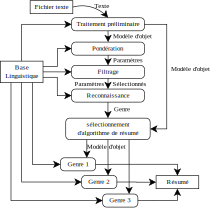
\includegraphics{RA/unis-model.pdf} %[width=140mm]
\caption[Le modèle général de UNIS]{Le modèle général de UNIS \cite{10-yatsko-al}.}
\label{fig:unis-model}
\end{center}
\end{figure}

%TODO done-ccl sur les outils industriels
Le résumé automatique est une nécessite ces jours à cause de bénéfices et des applications qu'on peut avoir en l'utilisant. 
Les outils que nous avons cités parmi autres, sont des outils très utiles qui visent fournir l'utilisateur par des résumés satisfaisantes en se basant sur les technologies que nous avons vu dans ce chapitre. 
Ces outils gratuits ou commercialisés peuvent être d'une grande utilité pour l'utilisateur.

%========================01========================%
%==================================================%
\section{Conclusion}

Dans ce chapitre, nous avons présenté un état de l'art sur le résumé automatique. 
Dans un premier temps, nous avons présenté quelques définitions pour le résumé, afin de comprendre ce domaine. 
Un résumé automatique peut appartient à plusieurs classes ou types, puisque il existe plusieurs critères de classification. 
Donc, nous avons vu qu'on peut diviser ces critères selon le document d'entrée, le but, et le document de sortie. 
Nous avons conclu que le choix de la classe du résumé pour chaque critère peut affecter la méthode de résumé utilisée. 
Ainsi, il est important de spécifier les différentes classes de notre résumé avant de le développer. 
Pour comprendre la fonction de résumé d'une manière générale, sans introduire les différents types et approches existants, nous avons vu que le résumé a trois étapes fondamentales: l'identification des sujets, l'interprétation des sujets, et la génération de résumé. 
Ensuite, nous avons présenté les deux méthodes: statistiques; qui calcule l'importance des unités de document en se basant sur des statistiques menées sur des critères comme la fréquence des mots, etc., et la méthode linguistique qui utilise des méthodes plus profondes pour analyser le document d'entrée et obtenir une représentation de ce document qui va être utilisée pour générer le résumé. 
Nous avons présenté quelques applications de résumé automatique. 
%Le but principal de résumé automatique est d'aider les individus là où ils sont besoin de comprendre le contenu d'un document long, donc il existe des outils industriels qu'on peut utiliser. 
%Nous avons présenté quelques exemples de ces outils, soit commerciaux ou gratuits. 
Enfin, Nous avons présenté quelques outils industriels.

Le domaine de résumé automatique est très vaste, nous avons essayé de couvrir l'essentiel. 
%Le résumé automatique de textes est le plus remarquable parmi les types de résumé automatique, en se basant sur le médium. 
En analysant les deux approches statistique et linguistique, on peut dire que l'approche linguistique est très prometteuse, à ce stade, il n'existe pas encore d'outils TALN puissants et performants. 
Cependant, l'approche statistique n'exige pas de ressources et donne des résultats satisfaisants. 
Malgré sa faible qualité linguistique, l'approche statistique reste une approche très puissante, qui a prouvé son utilité, et spécialement pour les documents scientifiques qui, d'après \cite{58-luhn}, n'utilisent pas une langue complexe et les mots importants sont souvent répétés. 
%Dans le chapitre suivant
Dans le chapitre suivant, nous allons présenter l'approche statistique pour le résumé automatique de texte. 

%========================Le pied de chapitre=======================================
%==================================================================================
\ifx\wholebook\relax\else
 \clearpage
 \let\wholebook=\relax
 \appendix
 \appendixfile{acronyms.tex}
 \bibliographystyle{../use/ESIbib}
 \bibliography{../bib/RA}
 \end{document}
\fi
%==================================================================================
